%%% Local Variables:
%%% mode: latex
%%% TeX-master: t
%%% End:


\newcommand\desmeth{x^{(k+1)} = x^{(k)} + t^{(k)}\Delta x^{(k)}}
\newcommand\satis{{\bf \small s.t}.   f(x^{(k+1)}) < f(x^{(k)})}
\newcommand\xk[1]{x^{(#1)}}
\newcommand\bx{{\bf x}}

\subsection{}
\begin{frame}
  \frametitle{Unconstrained Optimization}
  \begin{itemize}
  \item Minimize $f(x)$;
  \item Where $f : \mathbb{R}^n \rightarrow \mathbb{R}$ is convex
    and twice differentiable;
  \item No additional constraints;
  \item Assume that unique minimum $x^*$ exists.
  \end{itemize}
\end{frame}

\begin{frame}
  \frametitle{General Principle}
  \begin{itemize}
  \item Objective: minimize $f(x)$
  \item Necessary and sufficient condition: $\nabla f(x^*) = 0$
    \begin{itemize}
    \item Solve analytically
    \item Iterative algorithms
    \end{itemize}
  \end{itemize}

  \begin{block}{ Iterative Algorithm:}
    $$\xk{0}, \xk{1}, ... \in \dom f$$
    $$k \rightarrow \infty, f(\xk{k}) < f(x^*) $$
  \end{block}

  \begin{block}{Descent Method:}
    $$\desmeth,  \satis$$
  \end{block}

\end{frame}


\begin{frame}
  \frametitle{General Descent Method}
  \begin{block}{Descent Method:}
    \begin{equation}
      \desmeth,  \satis
      \label{equation: descent}
    \end{equation}
  \end{block}

  \only<1>{
    \begin{greenblock}{Algorithm:}
      \begin{algorithm}[H]
        \small
        Given $\xk{0} \in \dom f$\;
        \Repeat{$\Delta x$ is within an acceptable range and is stable;}{
          Determine a descent direction $\Delta x$\;
          Choose a step size $t > 0$\;
          Update $\desmeth$\;
        }
        % \caption{Descent Method Algorithm}
      \end{algorithm}
    \end{greenblock}
  }

  \only<2>{
    \begin{greenblock}{Theorem}
      \footnotesize
      For a continuously differentiable function $f$:
      $$f~ is~ convex \gdw f(x) \le f(y) + f'(y)(x - y)$$
    \end{greenblock}
    \vspace{-8pt}
    \begin{greyblock}{Proof}
      \footnotesize
      $$f(\xk{k+1}) \ge f(\xk{k}) + f'(\xk{k})\Delta \xk{k} $$
      $$\nabla f(\xk{k}) \le f(\xk(k+1)) - f(\xk{k}) < 0$$

    \end{greyblock}
  }

  \only<3>{
    \begin{greenblock}{Algorithm:}
      \begin{algorithm}[H]
        \small
        Given $\xk{0} \in \dom f$\;
        \Repeat{$\Delta x$ is within an acceptable range and is stable;}{
          Determine a descent direction $\Delta x$ $\Rightarrow$
          {$\footnotesize Gradient/Steepest Descent$}\;
          Choose a step size $t > 0$ $\Rightarrow$~~~~~~~~~~~~ $Line Search Algo$ \;
          Update $\desmeth$\;
        }
        % \caption{Descent Method Algorithm}
      \end{algorithm}
    \end{greenblock}
  }


  \begin{block}{Noticing that $f$ is convex:}
    \begin{equation}
      \label{eq:xconv}
      \nabla f(\xk{k})^T\Delta \xk{k} < 0
    \end{equation}
  \end{block}
\end{frame}


\begin{frame}
  \frametitle{Line Search}

  \only<1>{
    $\desmeth, f(\xk{k+1}) \leftarrow f(\xk{k})$
    \begin{columns}
      \begin{column}{0.5\textwidth}
        \centering
        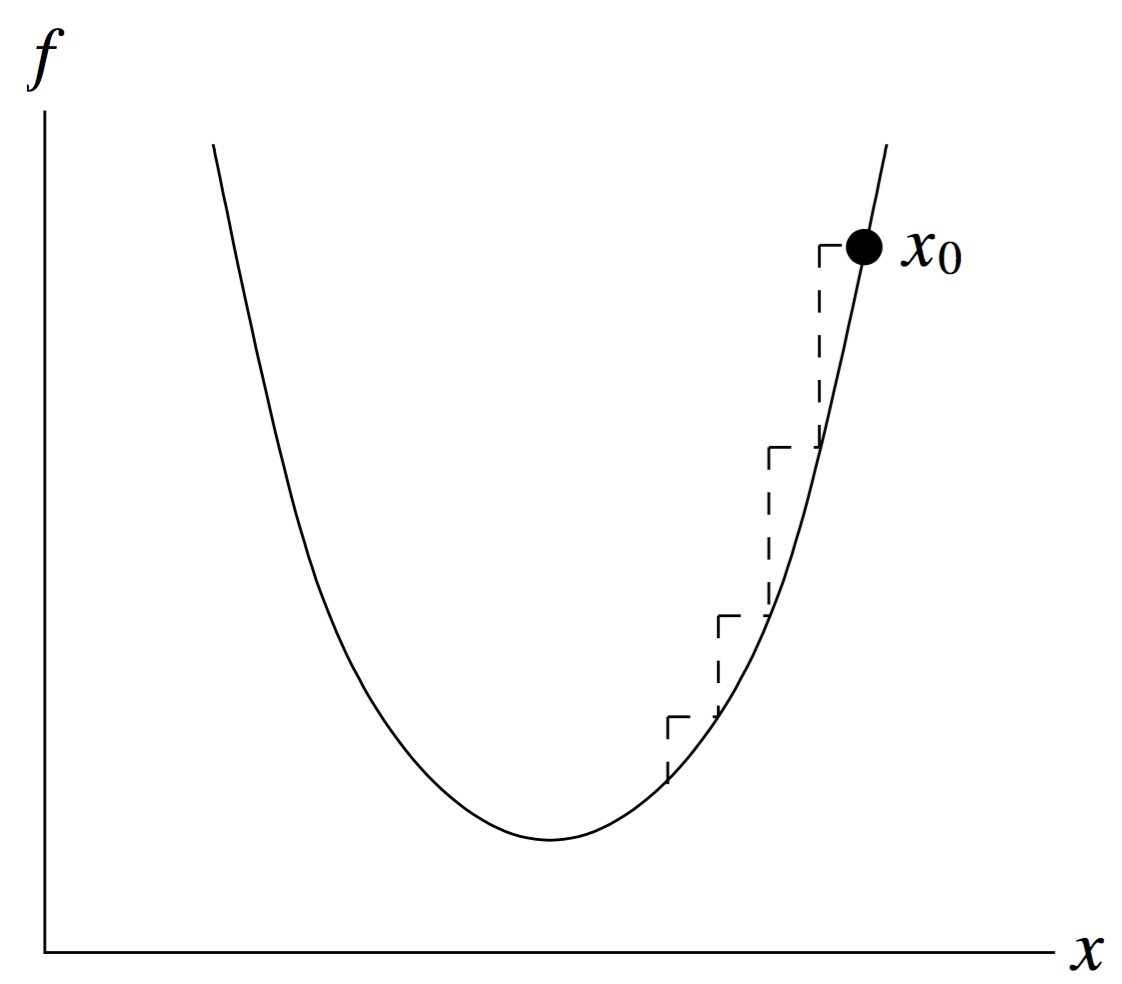
\includegraphics[scale=0.15]{pics/sa.png}

        {\tiny When Step Size t is Appropriate.}

        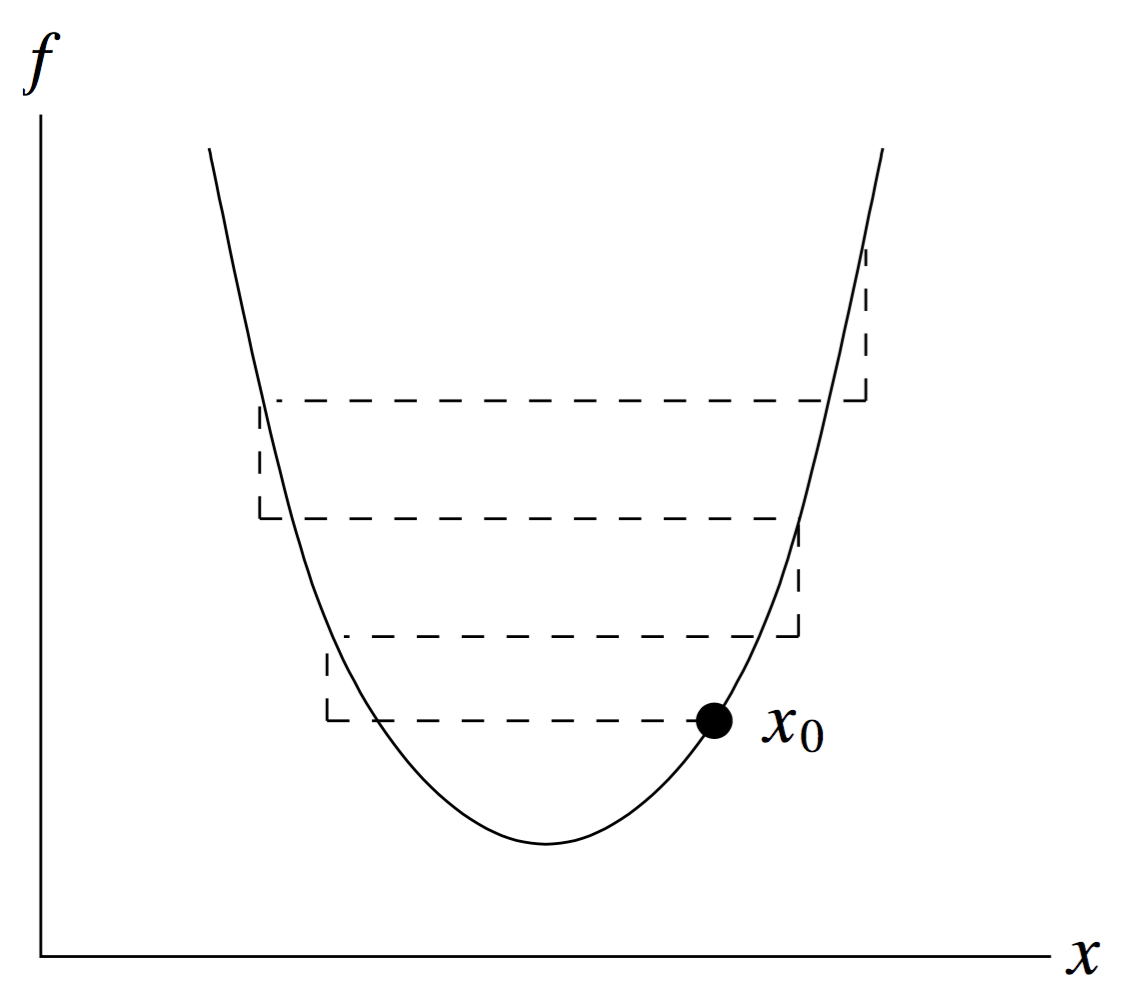
\includegraphics[scale=0.15]{pics/si.png}

        {\tiny When Step Size t is Inappropriate. }
      \end{column}


      \begin{column}{0.5\textwidth}
        \centering
        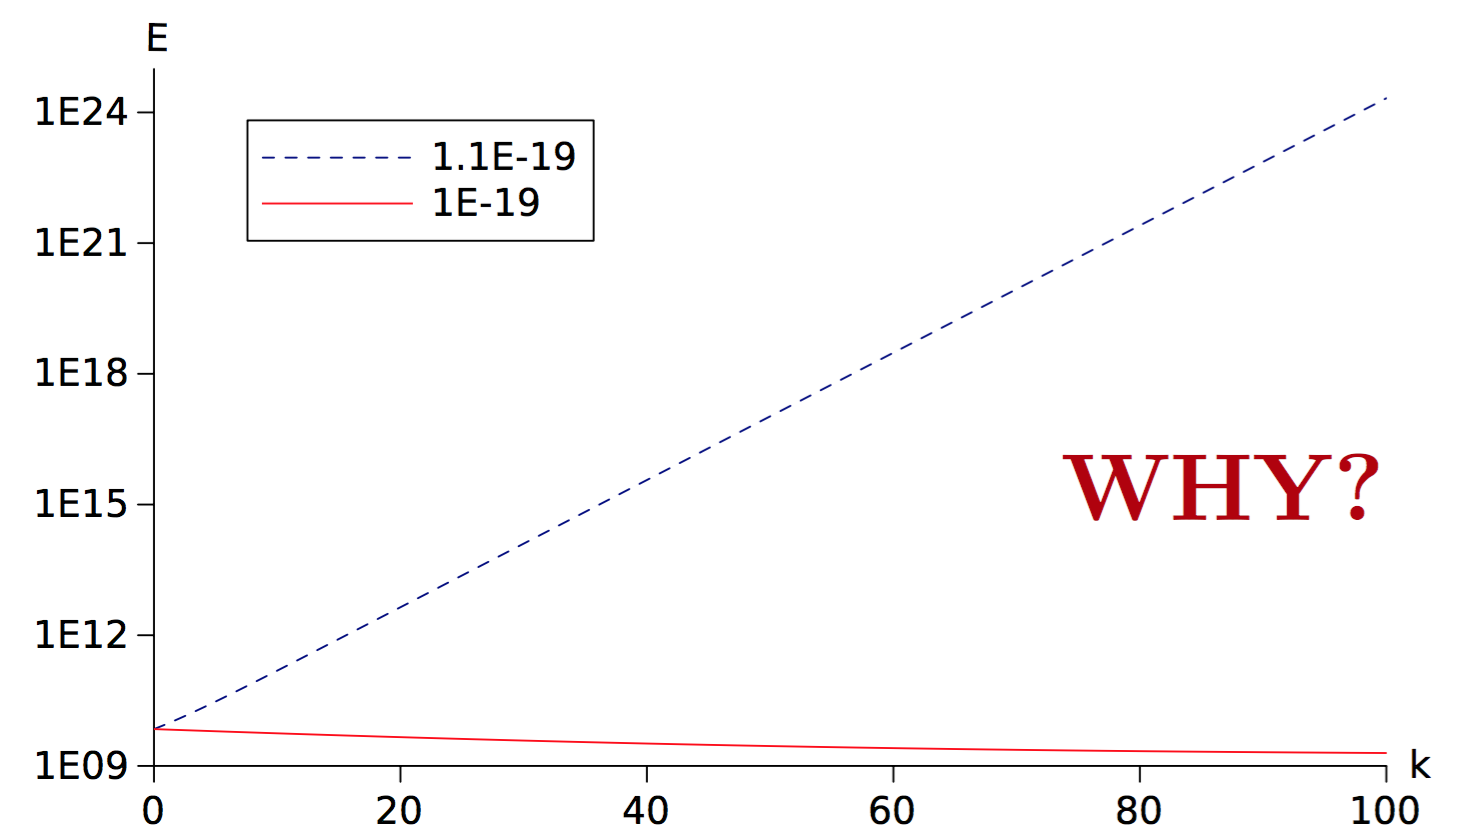
\includegraphics[scale=0.18]{pics/issue1.png}

        \vspace{4mm}

        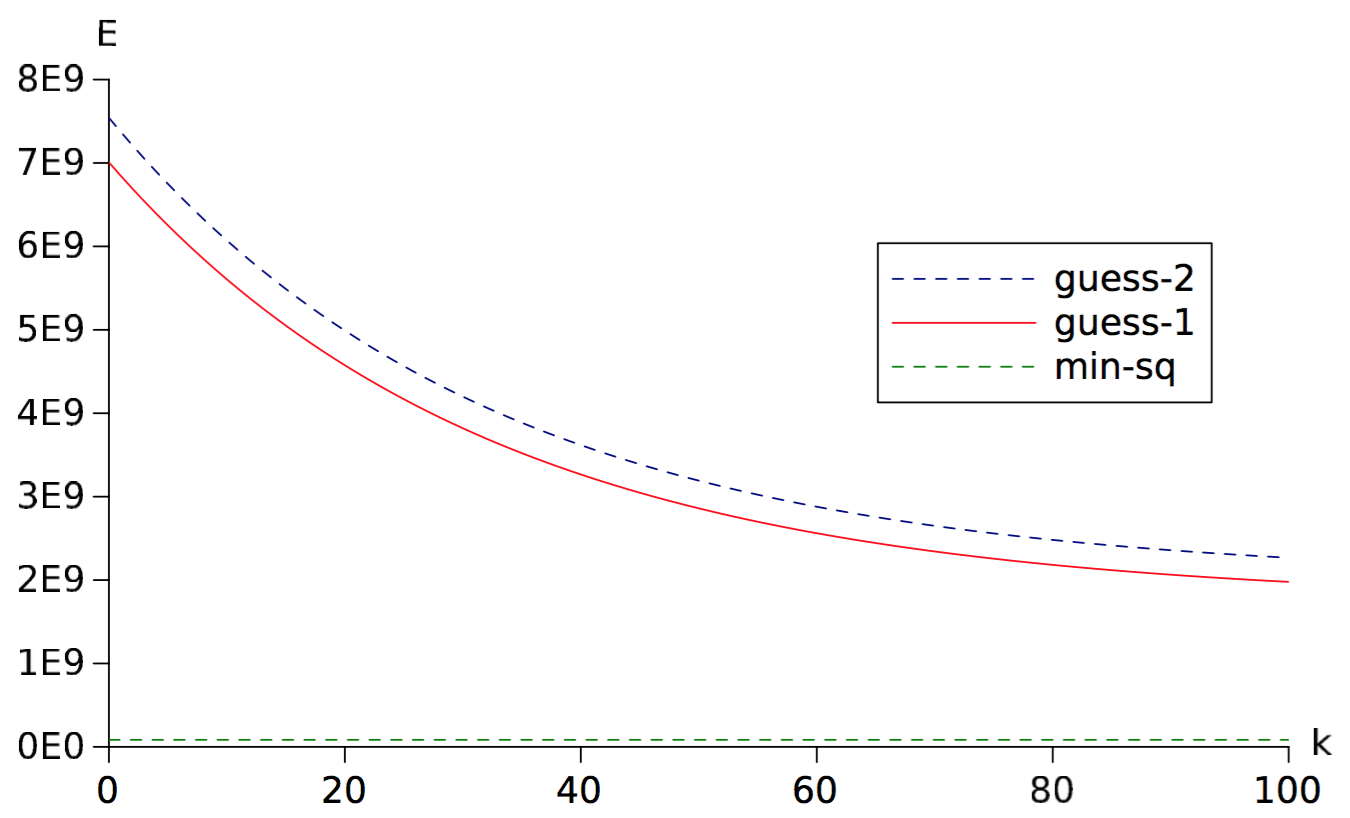
\includegraphics[scale=0.18]{pics/issue2.png}

      \end{column}
    \end{columns}
  }

  \only<2>{
    \begin{itemize}
    \item Armijo Condition:
      $$f(\xk{k} + t\Delta \xk{k}) \le f(\xk{k}) + c_1\alpha\nabla
      f(\xk{k})^T\Delta \xk{k}, c_1 > 0$$
    \item Wolfe Conditions (Including Armijo Condition):
      $$\nabla f(\xk{k} + t\Delta \xk{k})^Tp^{(k)} \ge c_2\nabla f(\xk{k})^Tp^{(k)}, 0< c_1 < c_2 < 1$$
    \end{itemize}
    \begin{greenblock}{Theorem:}
      Gradient descent will find local minimum if step size $\alpha$ satisfies Wolfe conditions.

    \end{greenblock}
  }

  \only<3>{
    \begin{itemize}
    \item Armijo Condition:
      $$f(\xk{k} + t\Delta \xk{k}) \le f(\xk{k}) + c_1\alpha\nabla
      f(\xk{k})^T\Delta \xk{k}, c_1 > 0$$
    \end{itemize}
    \begin{greenblock}{Algorithm:}
      \begin{algorithm}[H]
        \small
        Given a descent direction $\Delta x$ for $f$ at $x\in \dom f,
        \alpha \in (0, 0.5), \beta \in (0, 1), t = 1$\;
        \Repeat{$f(\xk{k} + t\Delta \xk{k}) \le f(\xk{k}) + c_1\alpha\nabla
          f(\xk{k})^T\Delta \xk{k}$;}{
          $t =\beta t$\;
        }
        % \caption{Descent Method Algorithm}
      \end{algorithm}
    \end{greenblock}
  {Exact Line Search Method:}
  $$\dis t = \argmin_{s\le 0}\{f(x + s\Delta x)\} $$
  }


\end{frame}

\begin{frame}
  \frametitle{General Descent Method}
  \begin{itemize}
  \item Gradient Descent Method
  \item Steepest Descent Method
  \end{itemize}
  $\Delta x$ satisfies:
  $$\nabla f(\xk{k})^T\Delta x < 0$$

\end{frame}


\begin{frame}
  \frametitle{Gradient Descent Method}
  \begin{greenblock}{$\Delta x = -\nabla f(x)$}
    \begin{algorithm}[H]
      \small
      Given $\xk{0} \in \dom f$\;
      \Repeat{$\Delta x$ is within an acceptable range and is stable;}{
        $\Delta x = -\nabla f(\xk{k})$\;
        Choose a step size $t > 0, [Line Search]$\;
        Update $x^{(k+1)} = x^{(k)}+ t\Delta x$\;
      }
      % \caption{Descent Method Algorithm}
    \end{algorithm}
  \end{greenblock}
\end{frame}

\begin{frame}
  \frametitle{Steepest Descent Method}
  % Determine a descent direction $\Delta x$

  \only<1>{
    $\Delta x = \Delta x_{sd}$

    Taylor Series:

    $$f(\bx + \Delta \bx) = f(\bx) + \nabla f(\bx)^T\Delta \bx +
    \frac{1}{2}\Delta\bx\nabla f(\bx)\Delta \bx$$

    $$f(\bx + {\bf v}) \approx \hat{f}(\bx + {\bf v}) = f(\bx) + \nabla
    f(\bx)^T{\bf v}$$

    $$\desmeth, \satis$$

    Where ${\bf v} $ is a descent direction if $\nabla f(\bx)^T < 0$
  }

  \only<2>{

    $$f(\bx + {\bf v}) \approx \hat{f}(\bx + {\bf v}) = f(\bx) + \nabla
    f(\bx)^T{\bf v}$$

    Normalized Steepest Descent Direction:
    \begin{equation}
      \begin{split}
        \Delta \bx_{nsd} & = \argmin\{\nabla f(\bx)^T{\bf v} | \norm{\bf v} = 1\} \\
        & =  \argmin\{\nabla f(\bx)^T{\bf v} | \norm{\bf v} \le 1\}
      \end{split}
    \end{equation}

  }

  \only<3>{
    Dual Norm, denoted $\norm{\cdot}_*$, is defined as:
    $$\norm{z}_* = sup\{z^Tx | \norm{x}\le 1\}$$

    Unnormalized Steepest Descent Direction:
    $$\Delta \bx = \norm{\nabla f(x)}_* \cdot \Delta \bx_{nsd}$$
    \begin{columns}
      \begin{column}{0.4\textwidth}
        \footnotesize
        \begin{equation*}
          \label{eq:some}
          \begin{split}
            \nabla f(\bx)^T{\bf v} & = \nabla f(\bx)^T\Delta\bx_{sd} \\
            & =\norm{f(x)}_*\nabla f(\bx)^T\Delta\bx_{nsd} \\
            & = -\norm{\nabla f{(x)}}^2_*
          \end{split}
        \end{equation*}
      \end{column}
      \begin{column}{0.6\textwidth}
        \footnotesize
        \begin{greenblock}{Proof}
          \begin{equation*}
            \begin{split}
              \Delta \bx_{nsd} & = \argmin\{\nabla f(\bx)^T{\bf v} | \norm{v} = 1\} \\
              & = - \argmax\{\nabla f(\bx)^T{\bf v} | \norm{v} \le 1\}
            \end{split}
          \end{equation*}
          \begin{equation*}
            \begin{split}
              \norm{\nabla f{(x)}}^2_* & = sup\{\nabla f(\bx)^T{\bf v} |
              \norm{v} \le 1 \} \\
              \Rightarrow \norm{\nabla f{(x)}}^2_* & = -\nabla f(\bx)^T\Delta x_{nsd}
            \end{split}
          \end{equation*}
        \end{greenblock}
      \end{column}
    \end{columns}

  }

  \only<4>{
    $\Delta \bx_{nsd}  = \argmin\{\nabla f(\bx)^T{\bf v} | \norm{\bf v} \le
    1\}$

    $\Delta \bx_{sd} = \norm{\nabla f(\bx)}_*\Delta \bx_{nsd}$

    \begin{greenblock}{Steepest Descent Method}
      \begin{algorithm}[H]
        \small
        Given $\xk{0} \in \dom f$\;
        \Repeat{$\Delta x$ is within an acceptable range and is stable}{
          Compute steepest descent direction $\Delta x_{sd}$\;
          Choose a step size $t > 0, [Line Search]$\;
          Update $x^{(k+1)} = x^{(k)} + t^{(k)}\Delta x^{(k)}_{sd}$\;
        }
        % \caption{Descent Method Algorithm}
      \end{algorithm}
    \end{greenblock}
  }

\end{frame}



\begin{frame}
  \frametitle{Descent Method}

\only<1>{
  \begin{blueblock}{General}
    \begin{algorithm}[H]
      \tiny
      Given $\xk{0} \in \dom f$\;
      \Repeat{$\Delta x$ is within an acceptable range and is stable}{
        Determine a descent direction $\Delta x$\;
        Choose a step size $t > 0$\;
        Update $\desmeth$\;
      }
      % \caption{Descent Method Algorithm}
    \end{algorithm}
  \end{blueblock}
}

\only<2>{
  \begin{blueblock}{General}
  \begin{itemize}
  \item $\Delta \bx_{nsd}  = \argmin\{\nabla f(\bx)^T{\bf v} | \norm{\bf v} \le
    1\} $
  \item $\Delta\bx_{sd} = \norm{\nabla f(x)}_*\cdot \Delta \bx_{nsd}$
  \item If the norm $\norm{\cdot}$ is Euclidean norm, $\Delta \bx =
    -\nabla f(\bx)$
  \end{itemize}
  \end{blueblock}
\vspace{2mm}

}


  \begin{columns}[t]
    \begin{column}{0.5\textwidth}
      \begin{greenblock}{Gradient Descent}
        \begin{algorithm}[H]
          \tiny
          Given $\xk{0} \in \dom f$\;
          \Repeat{$\Delta x$ is within an acceptable range and is stable}{
          $\Delta x = -\nabla f(\xk{k})$\;
          Choose a step size $t > 0, [Line Search]$\;
          Update $x^{(k+1)} = x^{(k)}+ t\Delta x$\;
        }

        \end{algorithm}

      \end{greenblock}
    \end{column}

    \begin{column}{0.5\textwidth}
      \begin{greenblock}{Steepest Descent}
        \begin{algorithm}[H]
          \tiny
          Given $\xk{0} \in \dom f$\;
          \Repeat{$\Delta x$ is within an acceptable range and is stable}{
          Compute steepest descent direction $\Delta x_{sd}$\;
          Choose a step size $t > 0, [Line Search]$\;
          Update $x^{(k+1)} = x^{(k)} + t^{(k)}\Delta x^{(k)}_{sd}$\;
        }


        \end{algorithm}
        %   \small
        %   Given $\xk{0} \in \dom f$\;
        %   \Repeat{$\Delta x$ is within an acceptable range and is stable;}{
        %   Compute steepest descent direction $\Delta x_{sd}$\;
        %   Choose a step size $t > 0, [Line Search]$\;
        %   Update $x^{(k+1)} = x^{(k)} + t^{(k)}\Delta x^{(k)}_{sd}$\;
        % }

      \end{greenblock}

    \end{column}

  \end{columns}

\end{frame}

% \begin{frame}
%   \frametitle{Steepest Descent Method}
%   \begin{block}
%     \begin{algorithm}[H]
%       \small
%       Given $\xk{0} \in \dom f$\;
%       \Repeat{$\Delta x$ is within an acceptable range and is stable}{
%       Determine a descent direction $\Delta x$\;
%       Choose a step size $t > 0$\;
%       Update $\desmeth$\;
%     }
%       %       \caption{Descent Method Algorithm}
%     \end{algorithm}
%   \end{block}

%   \begin{columns}
%     \begin{column}{0.5\textwidth}
%       \begin{greenblock}
%         \begin{algorithm}[H]
%           \small
%           Given $\xk{0} \in \dom f$\;
%           \Repeat{$\Delta x$ is within an acceptable range and is stable}{
%           $\Delta x = -\nabla f(\xk{k})$\;
%           Choose a step size $t > 0, [Line Search]$\;
%           Update $x^{(k+1)} = x^{(k)}+ t\Delta x$\;
%         }

%         \end{algorithm}
%       \end{greenblock}
%     \end{column}

%     \begin{column}{0.5\textwidth}
%       \begin{greenblock}
%         \begin{algorithm}[H]
%           \small
%           Given $\xk{0} \in \dom f$\;
%           \Repeat{$\Delta x$ is within an acceptable range and is stable;}{
%           Compute steepest descent direction $\Delta x_{sd}$\;
%           Choose a step size $t > 0, [Line Search]$\;
%           Update $x^{(k+1)} = x^{(k)} + t^{(k)}\Delta x^{(k)}_{sd}$\;
%         }

%         \end{algorithm}
%       \end{greenblock}
%     \end{column}

%   \end{columns}

% \end{frame}
